\documentclass[conference]{IEEEtran}
\IEEEoverridecommandlockouts
% The preceding line is only needed to identify funding in the first footnote. If that is unneeded, please comment it out.
\usepackage{cite}
\usepackage{amsmath,amssymb,amsfonts}
\usepackage{algorithmic}
\usepackage{graphicx}
\usepackage{textcomp}
\usepackage{xcolor}
\usepackage[labelformat=empty]{caption}
\def\BibTeX{{\rm B\kern-.05em{\sc i\kern-.025em b}\kern-.08em
    T\kern-.1667em\lower.7ex\hbox{E}\kern-.125emX}}
\begin{document}

\title{Analisis Perbandingan Pola Arsitektur MVI vs. MVVM: Evaluasi Kinerja\\
}

\author{\IEEEauthorblockN{1\textsuperscript{st} Yohanes Kenny}
\IEEEauthorblockA{\textit{Pradita University} \\
\textit{Tangerang, Indonesia} \\
yohanes.kenny@student.pradita.ac.id}

\and
\IEEEauthorblockN{2\textsuperscript{nd} Muhammad Abdi Reinanda}
\IEEEauthorblockA{\textit{Pradita University} \\
\textit{Tangerang, Indonesia}\\
muhammad.abdi@student.pradita.ac.id}

\and
\IEEEauthorblockN{3\textsuperscript{rd} Joaquin Camilo Tololiu}
\IEEEauthorblockA{\textit{Pradita University} \\
\textit{Tangerang, Indonesia}\\
joaquin.camilo@student.pradita.ac.id}

\and
\IEEEauthorblockN{4\textsuperscript{th} Revaldo Sugianto}
\IEEEauthorblockA{\textit{Pradita University} \\
\textit{Tangerang, Indonesia}\\
revaldo.sugianto@student.pradita.ac.id}

\and
\IEEEauthorblockN{5\textsuperscript{th} Ronald Bryan Alfredo}
\IEEEauthorblockA{\textit{Pradita University} \\
\textit{Tangerang, Indonesia}\\ 
ronald.bryan@student.pradita.ac.id}

}

\maketitle

\begin{abstract}
Lorem Ipsum is simply dummy text of the printing and typesetting industry. Lorem Ipsum has been the industry's standard dummy text ever since the 1500s, when an unknown printer took a galley of type and scrambled it to make a type specimen book. It has survived not only five centuries, but also the leap into electronic typesetting, remaining essentially unchanged. It was popularised in the 1960s with the release of Letraset sheets containing Lorem Ipsum passages, and more recently with desktop publishing software like Aldus PageMaker including versions of Lorem Ipsum.
\end{abstract}

\begin{IEEEkeywords}
MVI, MVVM, pola arsitektur, evaluasi kinerja, kecepatan, memori.
\end{IEEEkeywords}

\section{Pendahuluan}

\textbf{\textcolor{red}{Pendahuluan kurang panjang, tambahkan seperti sejarah MVVM sejarah MVI ataupun hal lain sebagai landasan mengapa penelitian ini dilakukan}}

Dalam pengembangan perangkat lunak, pemilihan pola arsitektur yang tepat memainkan peran krusial dalam menentukan kualitas, keterbacaan, dan kinerja keseluruhan aplikasi. Dua pola arsitektur yang sering dibandingkan adalah Model-View-Intent (MVI) dan Model-View-ViewModel (MVVM). MVI menekankan pada unidirectional data flow dan pengelolaan kejadian (events), sementara MVVM fokus pada pemisahan antara tampilan (view) dan 
logika bisnis (view model). \\
\indent Penelitian ini bertujuan untuk mengidentifikasi dan memahami perbedaan kinerja antara MVI dan MVVM dalam konteks pengembangan aplikasi Android. Tujuan utama dari eksperimen ini adalah untuk mengevaluasi dan membandingkan performa kedua pola arsitektur tersebut dalam aspek kecepatan dan penggunaan memori. Dengan pemahaman yang mendalam tentang kelebihan dan kekurangan masing-masing pendekatan, pengembang perangkat lunak akan dapat membuat keputusan yang lebih terinformasi dalam memilih pola arsitektur yang sesuai dengan kebutuhan aplikasi mereka. \\
\indent Melalui eksperimen ini, kami berharap dapat memberikan kontribusi yang berharga dalam penelitian tentang pola arsitektur perangkat lunak dan membantu pengembang untuk memilih pola arsitektur yang optimal sesuai dengan tujuan dan karakteristik proyek mereka.


\textbf{\textcolor{red}{Hindari pengunaan kata saya, kami, sebaiknya gunakan kata penulis}}


\section{Kajian Terkait}

\subsection{MVI}
\indent MVI adalah sebuah pola desain yang menitikberatkan pada abstraksi tugas View terhadap Model, sehingga dalam konteks ini, View dianggap sebagai representasi langsung dari Model.

\indent MVI menitikberatkan perannya pada Model sebagai Sumber Kebenaran dari View. Karena Model tidak memiliki perilaku dan mudah didistribusikan\cite{anhar2024analisis}, replikasi View dapat dilakukan tanpa memengaruhi keadaan (state) dari setiap salinan secara bersamaan.

\indent Pola MVI sepenuhnya menyerahkan proses representasi Model kepada View, terutama dalam konteks Fragment. Model yang diterima oleh Fragment dari ViewModel bersifat Immutable, menjadikan Model sebagai abstraksi dari View itu sendiri\cite{nunkesser2023choosing}. Meskipun pendekatan ini lebih sederhana dalam interaksi daripada MVVM, namun kelemahan MVI terletak pada kemungkinan sebagian Model berada di luar kendali Fragment. Hal ini menyebabkan Fragment kesulitan dalam mengubah Model tanpa melewati serangkaian proses yang kompleks. Perbedaan kewenangan antara Model dan Fragment juga sulit dideskripsikan secara jelas oleh Model itu sendiri, setidaknya sampai saat ini.

\begin{figure}[htp]
    \centering
    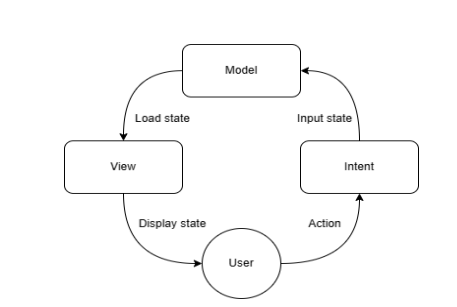
\includegraphics[width=7cm]{image/MVI.png}
    \caption{Gambar 1. Alur arsitektur MVI}
    \label{fig:mvi}
\end{figure}

\indent Salah satu keunggulan utama dari MVI adalah penerapan prinsip Single Source of Truth (SSOT), di mana kode inti ditempatkan dalam satu file. Hal ini menyebabkan penulisan program yang lebih sederhana dan dapat dimodifikasi dengan mudah, serta memastikan bahwa semua data dapat diakses dengan tepat, yang nantinya akan mempermudah proses perawatan (maintenance) di masa mendatang.\cite{arif2021optimasi}.MVI memiliki keunggulan yang unik dalam konsep Separation of Concernsnya, yang memungkinkan penyederhanaan manajemen keadaan (state management) dalam aplikasi program.

\subsection{MVVM}



\indent Model-View-View-Model (MVVM) adalah paradigma desain arsitektur baru untuk menangani persetujuan pengguna saat mengembangkan aplikasi Android yang berfungsi sebagai antarmuka pengguna (back-end \textbf{\textcolor{red}{antarmuka pengguna itu front end...}}). MVVM juga merupakan varian modern dari Model-View-Controller (MVC) dan tujuan intinya adalah memisahkan antara komponen Model dan komponen View\cite{rasyid2022sistem}. Sejak Google pertama kali mengumumkan MVVM pada Google I/O 2018, Google selalu mendorong setiap developer untuk mengerjakan aplikasi Android Studio.\cite{maulana2022aplikasi}

\indent ViewModel tidak dapat ditansaksikan. Hal ini memberikan konsekuensi dimana state dari View (secara design) tidak dapat dicopy atau didistribusikan \cite{saputro2020implementasi}. Oleh karena itu merepresentasikan ulang state dari View bisa menjadi sebuah tantangan. Walaupun secara teknis hal ini dapat dilakukan, Akan tetapi menggunakan Shared ViewModel yang Mutable membuat source of truth dipertanyakan kebenarannya.

\indent MVVM diclaim memudahkan kita untuk melakukan view management. Arsitektur MVVM memiliki keunggulan dalam modifiabilitas\cite{anhar2024analisis}. Dengan ViewModel mengatakan pada Fragment bagaimana dia harus merepresentasikan model, manajemen View memang bisa menjadi lebih mudah. Akan tetapi hal ini kadang membuat ViewModel menjadi bulky dan complex. Bahkan bisa lebih kompleks lagi jika kita berbicara mengenai Shared ViewModel. Konsekuensi dan batasan bagaimana ViewModel harus berperilaku seringnya tidak jelas. Secara prinsib, Fragment seharusnya tidak perlu lagi memikirkan bagaimana View harus di representasikan, akan tetapi pada praktiknya, beberapa Event dan Interaksi yang kompleks lebih mudah dihandle langsung oleh Fragment tanpa melalui ViewModel. Hal tersebut menjadi Gray Area antara tugas Fragment dan ViewModel vs Effort dan Kompleksitas, dan pada akhirnya kita memiliki 2 buah class yakni Fragment dan ViewModel yang sama-sama kompleks, dengan Gray Area yang dilematis. 

Komponen dalam MVVM adalah:
\begin{enumerate}
  \item Model \\
  Bagian ini mewakili inti dari logika bisnis dan data. Ini berarti bahwa logika bisnis menentukan cara data dimanipulasi dan disimpan dalam Model\cite{rasyid2022sistem}.
  
  \item View \\
  Komponen ini merupakan representasi antarmuka pengguna dan pada dasarnya berisi elemen antarmuka seperti layout XML dan sejenisnya\cite{rasyid2022sistem}.
  
  \item ViewModel \\
  ViewModel adalah elemen kunci dalam arsitektur ini karena membantu memisahkan tampilan dari logika bisnis. Ini bertindak sebagai penghubung antara View dan Model, menjaga keduanya terpisah namun memungkinkan interaksi dan koordinasi di antara keduanya. ViewModel juga menyimpan instruksi dan metode untuk mempertahankan status tampilan dan mengelola Model sesuai dengan tindakan yang dilakukan pada View. Selain itu, ViewModel juga memfasilitasi pemicuan peristiwa di dalam View itu sendiri\cite{rasyid2022sistem}.
\end{enumerate}


\begin{figure}[htp]
    \centering
    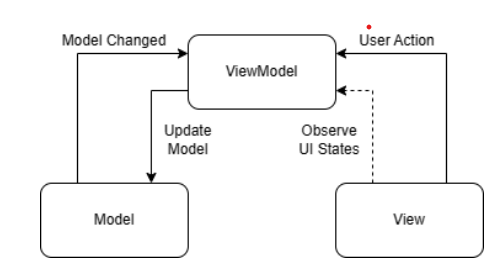
\includegraphics[width=7cm]{image/MVVM.png}
    \caption{Gambar 1. Alur arsitektur MVVM}
    \label{fig:mvi}
\end{figure}


\section{Metodologi}
Lorem Ipsum is simply dummy text of the printing and typesetting industry. Lorem Ipsum has been the industry's standard dummy text ever since the 1500s, when an unknown printer took a galley of type and scrambled it to make a type specimen book. It has survived not only five centuries, but also the leap into electronic typesetting, remaining essentially unchanged. It was popularised in the 1960s with the release of Letraset sheets containing Lorem Ipsum passages, and more recently with desktop publishing software like Aldus PageMaker including versions of Lorem Ipsum.

\bibliographystyle{plain}
\bibliography{reference}

\vspace{12pt}
\end{document}
